\section{精确惩罚法}
\label{sec:pm-exact}

上一节的二次罚必须把$\rho$推向无穷，原因就在罚项本身：平方函数在零点的斜率是零。可行边界上，罚项完全没有回推的力，目标只要有一点斜率，点就会越过边界，直到弹簧被拉长。这就需要回答：换一种在边界上就有斜率的罚项，有限的$\rho$能否直接得到原问题的解？

\paragraph{一次罚函数}
把平方换成绝对值和正部本身，在零点就有了尖角：

\begin{definition}[一次罚函数]
\label{def:pm-exact-penalty}
对问题~\eqref{eq:pm-problem}和$\rho>0$，记总违规量
\begin{equation}
 V(\bm{x})=\sum_{i=1}^m[g_i(\bm{x})]_++\sum_{j=1}^p\lvert h_j(\bm{x})\rvert ,
 \label{eq:pm-total-violation}
\end{equation}
称
\begin{equation}
 E_\rho(\bm{x})=f(\bm{x})+\rho V(\bm{x})
 \label{eq:pm-exact-penalty}
\end{equation}
为\term{一次罚函数}（$\ell_1$ penalty function）。若存在有限的$\rho$，使$E_\rho$的最小点就是原问题的最小点，就称这个罚函数是\term{精确罚函数}（exact penalty function）。
\end{definition}

“精确”说的是两个问题的解之间的对应关系。它并不表示数值上已经把子问题解到了机器精度，也不表示算法可以一步得到解。

\begin{example}[一维例的一次罚]
\label{ex:pm-exact-one-dim}
式~\eqref{eq:pm-one-dim}的一次罚函数是
\[
 E_\rho(x)=x+\rho[1-x]_+ .
\]
$x>1$时斜率是$1$，$x<1$时斜率是$1-\rho$。结果按$\rho$分成三种情形：
\begin{itemize}
 \item $\rho<1$时，$x<1$的一侧斜率为正，$x\to-\infty$时$E_\rho\to-\infty$，没有最小点；
 \item $\rho=1$时，$x\leq1$的整条射线上$E_\rho\equiv1$，最小点集合比原问题的解大；
 \item $\rho>1$时，$E_\rho$在$x=1$处由负斜率转为正斜率，$x=1$是唯一最小点。
\end{itemize}
门槛恰好是$\lambda^\star=1$。
\end{example}

图~\ref{fig:pm-exact-1d}(a)画出这三种情形。尖角的作用从图上一眼可见：只要左边的斜率足够陡，最低点就被“钉”在尖角上，不需要$\rho$继续增大。这和一元绝对值函数的最小点停在零点，是同一种机制。

\begin{BookInlineFigure}
  \centering
  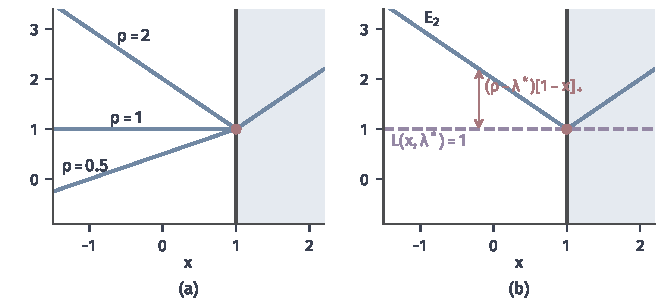
\includegraphics[width=112mm]{figures/05-optimization/06-constrained-optimization/matplotlib/pm-exact-1d/figure.pdf}
  \caption{一维例的一次罚函数。浅蓝区域可行，深灰竖线是约束边界，红点是解$x^\star=1$。(a)蓝线是$\rho=0.5,1,2$的$E_\rho$：$\rho<1$无下界，$\rho=1$左侧水平，$\rho>1$最小点就是$x^\star$。(b)蓝线是$E_2$，紫色虚线是Lagrange函数$\mathcal{L}(x,\lambda^\star)\equiv1$，$E_2$在它上方，红色箭头是两者之差。}
  \label{fig:pm-exact-1d}
\end{BookInlineFigure}

\paragraph{二元例的比较}
式~\eqref{eq:pm-running}的一次罚函数是
\[
 E_\rho(\bm{x})=\frac12x_1^2+\frac32x_2^2+\rho\lvert x_1+x_2-4\rvert .
\]
最优性条件是存在$\xi\in\partial\lvert\cdot\rvert(h(\bm{x}))$，使$\bm{x}$满足
\[
 x_1+\rho\xi=0,\qquad 3x_2+\rho\xi=0 .
\]
其中$\xi=\operatorname{sign}(h)$（当$h\neq0$），$\xi\in[-1,1]$（当$h=0$）。先假设解落在$h<0$的一侧，此时$\xi=-1$，解出
\[
 \bm{x}=\rho\Bigl(1,\ \frac13\Bigr).
\]
$h<0$要求$\tfrac43\rho-4<0$，即$\rho<3$。当$\rho\geq3$时，取$h=0$，也就是$\bm{x}=(3,1)$，由第一个方程得
\[
 \xi=-\frac{3}{\rho}\in[-1,0).
\]
所以$\rho\geq3$时解就是$\bm{x}^\star$，门槛是$\lvert\nu^\star\rvert=3$。

图~\ref{fig:pm-exact-path}把两种罚放在同一张图里。二次罚的$x_1(\rho)$永远在逼近$3$而到不了；一次罚先沿直线上升，在$\rho=3$处到达$3$，此后不再变化，违规量恰好为零。代价是$\rho<3$时一次罚的违规量可能更大，并且$E_\rho$在解处不可微。

\begin{BookInlineFigure}
  \centering
  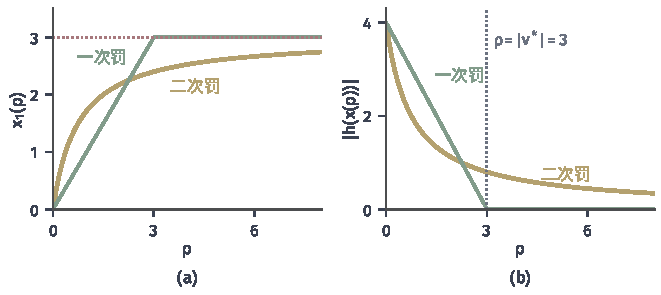
\includegraphics[width=112mm]{figures/05-optimization/06-constrained-optimization/matplotlib/pm-exact-path/figure.pdf}
  \caption{二元例中两种罚函数的解随$\rho$变化。黄线是二次罚，绿线是一次罚，(a)中红色点线是$x_1^\star=3$。(a)第一个坐标：二次罚只能渐近，一次罚在$\rho=3$到达并停住。(b)违规量：一次罚在$\rho\geq3$时恰为零，门槛等于$\lvert\nu^\star\rvert$。}
  \label{fig:pm-exact-path}
\end{BookInlineFigure}

\begin{BookInlineTable}
  \centering
  \begin{tabular}{@{}lll@{}}
    \toprule
     & 二次罚$Q_\rho$ & 一次罚$E_\rho$\\
    \midrule
    边界上的斜率 & 零 & 非零\\
    有限$\rho$的解 & 一般不可行 & 超过门槛后可行\\
    光滑性 & 一阶连续可微 & 边界上不可微\\
    $\rho$的取法 & 必须趋于无穷 & 只需超过乘子门槛\\
    内层困难 & 法向曲率增长 & 解处有尖角\\
    \bottomrule
  \end{tabular}
  \caption{二次罚与一次罚的对照。二次罚以病态换取光滑，一次罚以不可微换取有限的罚参数。}
  \label{tab:pm-penalty-contrast}
\end{BookInlineTable}

\subsection{精确性的条件}
\label{sec:pm-exact-conditions}

门槛和乘子的关系不是例子的巧合。下面要把它写成定理，并分清全局和局部两个层次。

\paragraph{全局精确性}
回忆第~\ref{chap:duality}章的记号。Lagrange函数是
\[
 \mathcal{L}(\bm{x},\bm{\lambda},\bm{\nu})=f(\bm{x})+\sum_{i=1}^m\lambda_ig_i(\bm{x})+\sum_{j=1}^p\nu_jh_j(\bm{x}),
\]
对偶函数$q$是$\mathcal{L}$对$\bm{x}$的下确界。弱对偶说$\bm{\lambda}\geq\bm{0}$时$q(\bm{\lambda},\bm{\nu})\leq f^\star$；强对偶说存在$(\bm{\lambda}^\star,\bm{\nu}^\star)$使等号成立。这个下界和一次罚函数放在一起，就是图~\ref{fig:pm-exact-1d}(b)的画面：$\mathcal{L}(x,\lambda^\star)$是整条水平线，$E_\rho$处处在它上方。

\begin{theorem}[一次罚的全局精确性]
\label{thm:pm-exact-global}
设原问题的最优解$\bm{x}^\star$存在，对偶问题的最优解$(\bm{\lambda}^\star,\bm{\nu}^\star)$存在，且强对偶成立，$q(\bm{\lambda}^\star,\bm{\nu}^\star)=f^\star$。若
\begin{equation}
 \rho>\max\Bigl\{\max_i\lambda_i^\star,\ \max_j\lvert\nu_j^\star\rvert\Bigr\},
 \label{eq:pm-exact-threshold}
\end{equation}
则$E_\rho$的全局最小点集合恰好等于原问题的全局最优解集合，且对所有$\bm{x}$有
\begin{equation}
 E_\rho(\bm{x})\geq f^\star+\delta V(\bm{x}),
 \label{eq:pm-exact-lower-bound}
\end{equation}
其中$\delta>0$是$\rho$与门槛之差。
\end{theorem}

\begin{proof}
记门槛为$\rho_0$，$\delta=\rho-\rho_0>0$。先建立式~\eqref{eq:pm-exact-lower-bound}。由$\lambda_i^\star\geq0$和$g_i\leq[g_i]_+$，有
\[
 \lambda_i^\star g_i(\bm{x})\leq\lambda_i^\star[g_i(\bm{x})]_+\leq\rho_0[g_i(\bm{x})]_+ .
\]
对等式项同样有
\[
 \nu_j^\star h_j(\bm{x})\leq\lvert\nu_j^\star\rvert\lvert h_j(\bm{x})\rvert\leq\rho_0\lvert h_j(\bm{x})\rvert .
\]
把这些不等式对$i,j$求和，得到
\[
 \sum_i\lambda_i^\star g_i(\bm{x})+\sum_j\nu_j^\star h_j(\bm{x})\leq\rho_0V(\bm{x}).
\]

于是
\[
 \begin{aligned}
 E_\rho(\bm{x})&=f(\bm{x})+\rho_0V(\bm{x})+\delta V(\bm{x})\\
 &\geq\mathcal{L}(\bm{x},\bm{\lambda}^\star,\bm{\nu}^\star)+\delta V(\bm{x})\\
 &\geq q(\bm{\lambda}^\star,\bm{\nu}^\star)+\delta V(\bm{x}).
 \end{aligned}
\]
由强对偶，最后一式等于$f^\star+\delta V(\bm{x})$，这就是式~\eqref{eq:pm-exact-lower-bound}。

再看最小点集合。任一原问题最优解$\bm{x}^\star$满足$V(\bm{x}^\star)=0$，$E_\rho(\bm{x}^\star)=f^\star$，由下界知它是$E_\rho$的全局最小点，且$E_\rho$的最小值是$f^\star$。

反过来，设$\bar{\bm{x}}$是$E_\rho$的全局最小点，则$E_\rho(\bar{\bm{x}})=f^\star$。代入下界得$\delta V(\bar{\bm{x}})\leq0$，所以$V(\bar{\bm{x}})=0$，$\bar{\bm{x}}$可行。此时$f(\bar{\bm{x}})=E_\rho(\bar{\bm{x}})=f^\star$，它是原问题的最优解。
\end{proof}

式~\eqref{eq:pm-exact-threshold}中的门槛用的是最大绝对分量，因为总违规量是$\ell_1$形式，两者互为对偶范数。门槛可以按任一组最优乘子计算，最优乘子不唯一时，取能使门槛最小的一组。

证明里没有用到凸性，全部负担都在强对偶上。对一般的非凸问题，强对偶很少成立，所以全局精确性主要是凸问题的结论；第~\ref{chap:duality}章给出的Slater条件是常用的充分条件。

严格不等号也不能省。一维例中$\rho=1$恰好等于门槛，$E_1$的最小点是整条射线$(-\infty,1]$，原问题的解只是其中一点。此时$\delta=0$，下界~\eqref{eq:pm-exact-lower-bound}里违规量的系数消失，最后一步推不出可行。

\paragraph{对偶解不存在时}
去掉“对偶最优解存在”，结论会彻底失败。考虑
\[
 \min_x\ x\qquad\text{s.t.}\qquad x^2\leq0 .
\]
可行集只有$\{0\}$，$x^\star=0$。这是凸问题，$q(\lambda)=-1/(4\lambda)$，$\lambda\to\infty$时趋于$0=f^\star$，但上确界取不到，不存在有限的最优乘子。它的一次罚是$E_\rho(x)=x+\rho x^2$，唯一最小点是
\[
 x_\rho=-\frac{1}{2\rho}\neq0 .
\]
对每个有限的$\rho$，最小点都不可行，$\rho$必须趋于无穷。这里约束的梯度在解处是零，违规量$x^2$在解处光滑，根本没有尖角。可见一次罚的尖角要靠约束的梯度才能起作用。

\paragraph{局部精确性}
非凸问题用不上强对偶，可以只问局部：$\bm{x}^\star$是否是$E_\rho$的局部最小点。局部分析有两条路线。一条看约束集的几何，要求违规量控制到可行集的距离；另一条看KKT条件和曲率。

第一条路线的条件是\term{局部误差界}（local error bound）：存在$\tau>0$和$\bm{x}^\star$的邻域，使邻域内的$\bm{x}$满足
\begin{equation}
 \operatorname{dist}(\bm{x},\bm{C})\leq\tau V(\bm{x}).
 \label{eq:pm-error-bound}
\end{equation}
它的意思是，违规量小就真的离可行集近，不会出现违规量几乎为零、点却还很远的情况。线性约束时误差界在整个空间成立，这是Hoffman界。对光滑约束，它在Mangasarian--Fromovitz约束资格下成立，证明需要用到非线性系统的度量正则性，篇幅较长，这里只使用结论。

第二条路线要用到二阶条件。在KKT点$(\bm{x}^\star,\bm{\lambda}^\star,\bm{\nu}^\star)$处，临界方向$\bm{d}$满足
\begin{equation}
 \nabla h_j(\bm{x}^\star)^\top\bm{d}=0,\qquad
 \begin{cases}
 \nabla g_i(\bm{x}^\star)^\top\bm{d}=0, & g_i(\bm{x}^\star)=0,\ \lambda_i^\star>0,\\
 \nabla g_i(\bm{x}^\star)^\top\bm{d}\leq0, & g_i(\bm{x}^\star)=0,\ \lambda_i^\star=0.
 \end{cases}
 \label{eq:pm-critical-cone}
\end{equation}
二阶充分条件要求Lagrange函数在KKT点处的Hessian沿每个非零临界方向$\bm{d}$都有正曲率：
\[
 \bm{d}^\top\nabla^2_{\bm{x}\bm{x}}\mathcal{L}(\bm{x}^\star,\bm{\lambda}^\star,\bm{\nu}^\star)\bm{d}>0 .
\]
它的含义第~\ref{chap:constrained-optimality}章已经建立。

\begin{theorem}[一次罚的局部精确性]
\label{thm:pm-exact-local}
设$\bm{x}^\star$是可行点。
\begin{enumerate}
 \item 设$\bm{C}$是闭集，$\bm{x}^\star$是$f$在$\bm{C}$上的局部最小点，$f$在$\bm{x}^\star$的邻域内$G$-Lipschitz，且局部误差界~\eqref{eq:pm-error-bound}成立。若$\rho>G\tau$，则$\bm{x}^\star$是$E_\rho$的局部最小点。
 \item 设$f,g_i,h_j$二阶连续可微，$(\bm{x}^\star,\bm{\lambda}^\star,\bm{\nu}^\star)$是KKT点并满足二阶充分条件。若$\rho$满足式~\eqref{eq:pm-exact-threshold}，则$\bm{x}^\star$是$E_\rho$的严格局部最小点。
\end{enumerate}
\end{theorem}

\begin{proof}
先证第一部分。取充分小的$r>0$，使$\lVert\bm{x}-\bm{x}^\star\rVert_2\leq r$时误差界成立，并使$\bm{x}^\star$在半径$2r$的球内是$f$在$\bm{C}$上的最小点，$f$在该球内$G$-Lipschitz。

任取这样的$\bm{x}$，设$\bm{y}$是$\bm{x}$在闭集$\bm{C}$上的一个最近点。$\bm{x}^\star$也在$\bm{C}$中，所以
\[
 \lVert\bm{x}-\bm{y}\rVert_2\leq\lVert\bm{x}-\bm{x}^\star\rVert_2\leq r .
\]
由三角不等式，$\bm{y}$在半径$2r$的球内。于是
\[
 f(\bm{x})\geq f(\bm{y})-G\lVert\bm{x}-\bm{y}\rVert_2\geq f(\bm{x}^\star)-G\tau V(\bm{x}).
\]
由此得
\[
 E_\rho(\bm{x})\geq f(\bm{x}^\star)+(\rho-G\tau)V(\bm{x})\geq E_\rho(\bm{x}^\star).
\]

再证第二部分，用反证法。设$\bm{x}^\star$不是严格局部最小点，则存在$\bm{x}^{(k)}\to\bm{x}^\star$，$\bm{x}^{(k)}\neq\bm{x}^\star$，$E_\rho(\bm{x}^{(k)})\leq f(\bm{x}^\star)$。记$\bm{d}^{(k)}=\bm{x}^{(k)}-\bm{x}^\star$，取子列使单位向量$\bm{d}^{(k)}/\lVert\bm{d}^{(k)}\rVert_2$收敛到$\bm{d}$。

记$\rho_0$为式~\eqref{eq:pm-exact-threshold}的右端，$\delta=\rho-\rho_0>0$，$[a]_-=\max\{-a,0\}$。对单个不等式约束，$a=g_i(\bm{x}^{(k)})$时有
\[
 \rho[a]_+-\lambda_i^\star a\geq\delta[a]_++\lambda_i^\star[a]_- .
\]
这个不等式分两种情形验证：$a>0$时左边等于$(\rho-\lambda_i^\star)a\geq\delta a$，$a\leq0$时左边等于$\lambda_i^\star\lvert a\rvert$。等式项类似，
\[
 \rho\lvert h_j\rvert-\nu_j^\star h_j\geq\delta\lvert h_j\rvert .
\]

把它们加起来，并用$\mathcal{L}^\star$表示乘子固定为$(\bm{\lambda}^\star,\bm{\nu}^\star)$的Lagrange函数，得到
\[
 E_\rho(\bm{x}^{(k)})\geq\mathcal{L}^\star(\bm{x}^{(k)})+\delta V(\bm{x}^{(k)})+\sum_i\lambda_i^\star[g_i(\bm{x}^{(k)})]_- .
\]
KKT条件给出$\mathcal{L}^\star(\bm{x}^\star)=f(\bm{x}^\star)$和$\nabla\mathcal{L}^\star(\bm{x}^\star)=\bm{0}$。作二阶展开，记$\bm{W}=\nabla^2\mathcal{L}^\star(\bm{x}^\star)$，则
\[
 \mathcal{L}^\star(\bm{x}^{(k)})=f(\bm{x}^\star)+\frac12(\bm{d}^{(k)})^\top\bm{W}\bm{d}^{(k)}+o(\lVert\bm{d}^{(k)}\rVert_2^2).
\]
结合$E_\rho(\bm{x}^{(k)})\leq f(\bm{x}^\star)$，得到
\[
 \delta V(\bm{x}^{(k)})+\sum_i\lambda_i^\star[g_i(\bm{x}^{(k)})]_-
 \leq-\frac12(\bm{d}^{(k)})^\top\bm{W}\bm{d}^{(k)}+o(\lVert\bm{d}^{(k)}\rVert_2^2).
\]

右边是$O(\lVert\bm{d}^{(k)}\rVert_2^2)$，所以左边每一项都是这个量级。展开$h_j(\bm{x}^{(k)})$，除以$\lVert\bm{d}^{(k)}\rVert_2$取极限，由$\lvert h_j\rvert=O(\lVert\bm{d}^{(k)}\rVert_2^2)$得$\nabla h_j(\bm{x}^\star)^\top\bm{d}=0$。对活动的$g_i$，$[g_i]_+=O(\lVert\bm{d}^{(k)}\rVert_2^2)$给出$\nabla g_i(\bm{x}^\star)^\top\bm{d}\leq0$；当$\lambda_i^\star>0$时，$[g_i]_-$也是这个量级，于是等号成立。所以$\bm{d}$是非零临界方向。

最后，上式左边非负。两边除以$\lVert\bm{d}^{(k)}\rVert_2^2$取极限，得到$\bm{d}^\top\bm{W}\bm{d}\leq0$，与二阶充分条件矛盾。
\end{proof}

两部分的结论都只说$\bm{x}^\star$附近的事。局部精确不等于全局精确，例如$\min-x^4$，约束$x=0$。此时$\nu^\star=0$，门槛是零，对任何$\rho>0$，$x=0$都是$E_\rho(x)=-x^4+\rho\lvert x\rvert$的严格局部最小点，而$x\to\infty$时$E_\rho\to-\infty$。

\subsection{非光滑罚问题的求解}
\label{sec:pm-exact-solve}

有了精确性，还要回答怎么解$E_\rho$。它的尖角恰好在解的位置上，光滑方法在这里不能直接使用。第~\ref{chap:nonsmooth-composite-optimization}章的工具可以逐一套用，但每种工具都要先核对问题的结构。

\paragraph{次梯度与最优性}
设$f$和$h_j$可微，问题是凸的。$0\in\partial E_\rho(\bm{x})$写开来，就是存在$\xi_j\in\partial\lvert\cdot\rvert(h_j(\bm{x}))$，使
\begin{equation}
 \nabla f(\bm{x})+\sum_{j=1}^p\rho\xi_j\nabla h_j(\bm{x})=\bm{0}.
 \label{eq:pm-exact-subgradient}
\end{equation}
和KKT的驻定方程比较，$\nu_j=\rho\xi_j$就是乘子估计。$\xi_j$落在$[-1,1]$内，$\lvert\nu_j\rvert\leq\rho$。如果解上某条约束的$\lvert\xi_j\rvert=1$且仍然违规，说明罚参数不够大，或者问题本身不可行。

次梯度法只需要这些$\xi_j$，但第~\ref{chap:nonsmooth-composite-optimization}章已经看到，步长固定时点会在尖角附近反复跳动，收敛很慢。图~\ref{fig:pm-exact-ista}里的黄线就是这种行为，它在约束直线两侧来回穿越，几乎每一步都不可行。

\paragraph{邻近梯度}
若把光滑部分$f$留给梯度步，把$\rho V$留给邻近步，就是第~\ref{chap:nonsmooth-composite-optimization}章的邻近梯度法。关键在于邻近映射能否算出。对二元例，设$\bm{a}=(1,1)$，$\tau=\alpha\rho$，要解的子问题是
\begin{equation}
 \bm{p}=\argmin_{\bm{x}}\ \frac12\lVert\bm{x}-\bm{v}\rVert_2^2+\tau\lvert\bm{a}^\top\bm{x}-4\rvert .
 \label{eq:pm-exact-prox}
\end{equation}
由最优性条件，存在$\lvert\cdot\rvert$在$\bm{a}^\top\bm{p}-4$处的次梯度$\xi$，使$\bm{p}=\bm{v}-\tau\xi\bm{a}$。两边与$\bm{a}$作内积，得到
\[
 \bm{a}^\top\bm{p}-4=\bm{a}^\top\bm{v}-4-\tau\xi\lVert\bm{a}\rVert_2^2 .
\]
令$s=(\bm{a}^\top\bm{v}-4)/\lVert\bm{a}\rVert_2^2$。若$\lvert s\rvert\leq\tau$，取$\xi=s/\tau$可使约束恰好满足，这时$\bm{p}$就是$\bm{v}$到直线的投影。若$\lvert s\rvert>\tau$，约束仍然违规，$\xi=\operatorname{sign}(s)$。两种情形合写成
\begin{equation}
 \bm{p}=\bm{v}-\operatorname{clip}_\tau(s)\,\bm{a},\qquad
 \operatorname{clip}_\tau(s)=\max\{-\tau,\min\{s,\tau\}\}.
 \label{eq:pm-exact-prox-solution}
\end{equation}

下面用这个公式走几步。取$\rho=4$，它大于门槛$3$。$f$的光滑常数是$3$，步长$\alpha=1/3$，所以$\tau=4/3$。迭代$\bm{v}=\bm{x}-\alpha\nabla f(\bm{x})$的两个坐标是$\tfrac23x_1$和$0$：
\[
 \bm{v}=\Bigl(x_1-\frac13x_1,\ x_2-x_2\Bigr)=\Bigl(\frac23x_1,\ 0\Bigr).
\]
从$\bm{x}^{(0)}=(0,0)$出发，$\bm{v}=(0,0)$，$s=-2$，被截断到$-\tau$，得到
\[
 \bm{x}^{(1)}=\Bigl(\frac43,\ \frac43\Bigr).
\]
第二步$\bm{v}=(\tfrac89,0)$，$s=-\tfrac{14}{9}$，仍被截断，得到
\[
 \bm{x}^{(2)}=\Bigl(\frac{20}{9},\ \frac43\Bigr).
\]
第三步$\bm{v}=(\tfrac{40}{27},0)$，$s=-\tfrac{34}{27}$，这次$\lvert s\rvert<\tau$，投影到直线上，得到
\[
 \bm{x}^{(3)}=\Bigl(\frac{74}{27},\ \frac{34}{27}\Bigr),\qquad h(\bm{x}^{(3)})=0 .
\]
此后每步都留在直线上，并沿直线逼近$(3,1)$。乘子估计可以从$\nu=\rho\xi=s/\alpha$读出，第三步是$-\tfrac{34}{9}\approx-3.78$，到解处变为$-3$。图~\ref{fig:pm-exact-ista}的绿线就是这条路径：有限步后恰好可行，这是尖角带来的好处，二次罚做不到。

\begin{BookInlineFigure}
  \centering
  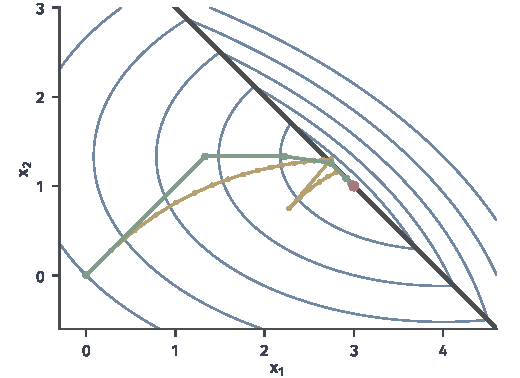
\includegraphics[width=88mm]{figures/05-optimization/06-constrained-optimization/matplotlib/pm-exact-ista/figure.pdf}
  \caption{二元例中一次罚$E_4$的两种解法，蓝线是等高线，深灰直线是约束。绿线是邻近梯度法（步长$1/3$），第三步落到直线上，此后沿直线走向红点。黄线是次梯度法（步长$0.07$），在直线两侧反复穿越，停留在解附近的一个小区域。}
  \label{fig:pm-exact-ista}
\end{BookInlineFigure}

\paragraph{一般约束的处理}
这个闭式解依赖约束只有一条且是线性的。若$\bm{h}(\bm{x})=\bm{A}\bm{x}-\bm{b}$有多行，$\lVert\bm{A}\bm{x}-\bm{b}\rVert_1$的邻近映射本身就要解一个优化问题；若$h_j$非线性，一般没有闭式解。

常用的办法是第~\ref{chap:nonsmooth-composite-optimization}章的局部模型：在当前点把约束线性化，保留绝对值，再加上二次距离项，解
\begin{equation}
 \min_{\bm{d}}\ \nabla f(\bm{x})^\top\bm{d}+\frac{1}{2\alpha}\lVert\bm{d}\rVert_2^2+\rho\sum_{j=1}^p\bigl\lvert h_j(\bm{x})+\nabla h_j(\bm{x})^\top\bm{d}\bigr\rvert .
 \label{eq:pm-exact-model}
\end{equation}
引入非负松弛变量把绝对值拆开，这是一个凸二次规划。模型是否可信要用真实的$E_\rho$检验，也就是比较预测下降和实际下降，第~\ref{chap:sequential-quadratic-programming}章会回到这一点。

解$E_\rho$结束时，还需要回到原问题做两项检查。第一，算出原约束的违规量$V(\bm{x})$，罚目标下降了不代表违规量已经降到容差以下。第二，核对$\rho$是否大于乘子估计的最大绝对分量。如果$\lvert\xi_j\rvert$贴着$1$，定理~\ref{thm:pm-exact-global}的条件就没有满足，应当增大$\rho$再解。数值上的$\rho$也不宜太大，否则目标的信息在罚项面前被淹没，迭代会贴着约束走得很慢。
